\section{Salze}

\subsection{Aufbau}
Salzartige Stoffe bestehen aus Kationen (oft Metallionen) und Anionen (\emph{immer} Nichtmetallionen). Ungerichtete elektrostatische Kräfte zwischen Ionen.\\

Ionische Bindung: Elektrostatische Wechselwirkungen zwischen allen Kationen und Anionen. $F = \frac{1}{4 \pi \epsilon_0} \cdot \frac{Q_1 + Q_2}{d^2}$ \\

Kristalline Stoffe, oft in dichtester Kugelpackung angeordnet, (abhängig von Ionengrösse und Ionenverhältnis) z.B. NaCl-Typ:
\begin{figure}[htbp]
	\centering
	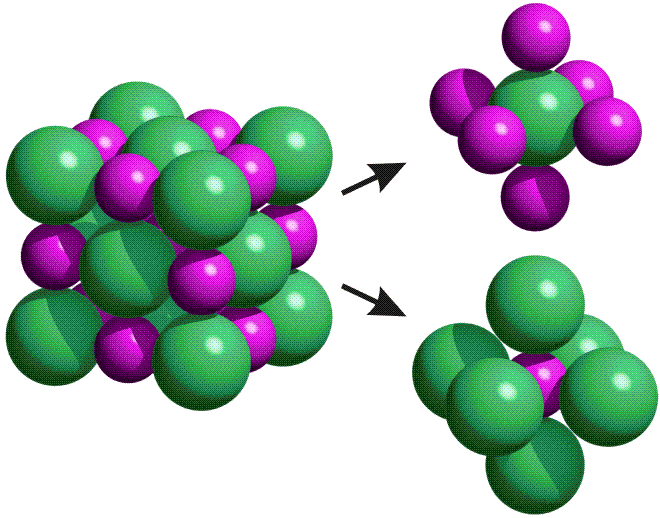
\includegraphics[width=0.5\linewidth]{images/5_Elementarzelle_NaCl.png}
\end{figure}

\subsection{Salzformel}
Verhältnisformeln. z.B. NaCl: Na$^+$ : Cl$^-$ = 1:1 \\

Bestimmung:
\begin{enumerate}
	\item Ionen erfüllen Edelgasregel $\Rightarrow$ Ionenladung der Elemente
	\item Salze sind insgesamt neutral
\end{enumerate}

\subsection{Nomenklatur}
Name Kation + (griech./lat.) Name Anion + \emph{-id} \\
Bei Übergangsmetallen: Kationenladung als römische Ziffer. \\

\subsection{Gitterenergie}
$E_G$: Energie, um ein Salz in seine freien Ionen zu zerlegen (bzw. umgekehrt). Vor allem durch Coulombkraft bestimmt: $E_G$ = f(Ionenladungen,Ionengrösse) \\

\subsection{Eigenschaften}
\subsubsection{Sprödigkeit}
Starke Wechselwirkung zwischen Ionen $\Rightarrow$ relativ hart. \\
Abstossung zwischen gleichartigen Ionen $\Rightarrow$ Sprödigkeit. \\
\begin{figure}[htbp]
	\centering
	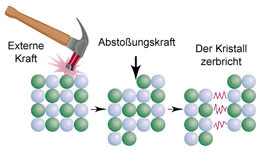
\includegraphics[width=0.5\linewidth]{images/5_Sproedigkeit.png}
\end{figure}

\subsubsection{Schmelz- und Siedepunkt}
Starke Wechselwirkungen $\Rightarrow$ hohe Schmelz- und Siedepunkte (Aufwendung der Gitterenergie $E_G$ notwendig $\Rightarrow$ abhängig von Ionenladung, Abstand, Grösse d. Ionen, Gittertyp). \\

\subsubsection{Elektrische Leitfähigkeit}
Als Feststoff: keine elektrische Leitfähigkeit, gelöst: gute Leitfähigkeit.

\subsubsection{Löslichkeit}
Viele Salze gut wasserlöslich (nur mit polaren Lösungsmitteln). \\
Vorgang:
\begin{enumerate}
	\item Oberflächen-Ionen ziehen Dipolmoleküle ($\delta+,\delta-$) an
	\item Ablösen und Hydration der Ionen.
\end{enumerate}
Schreibweise: $NaCl_{(s)} \, \rightarrow \, Na^+_{(aq)} + Cl^-_{(aq)}$ \\

Abschätzen: Löslichkeit ~ $E_G$ ~ Ionenladung und Ionengrösse
\begin{figure}[htbp]
	\centering
	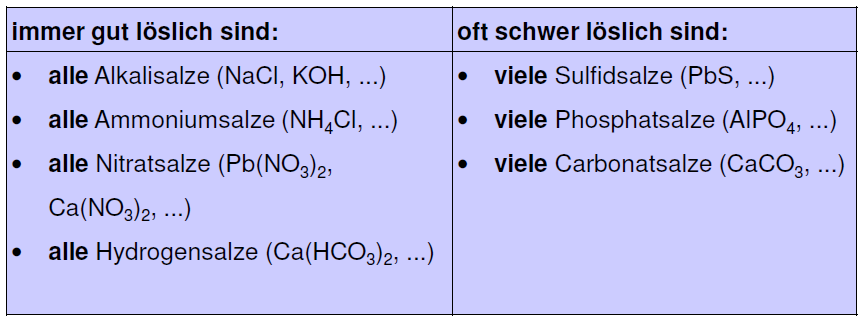
\includegraphics[width=0.9\linewidth]{images/5_Tabelle_Loeslichkeit.png}
\end{figure}